\chapter{Sistema de comunicación}

Una vez habíamos creado el sistema de observaciones, quedaba que los agentes pudieran controlar a los jugadores del entorno. Pero para hacer esto surgía el mismo problema que con las observaciones, es necesario realizar una comunicación entre el proceso de Python y el videojuego.

La primera idea que apareció fue usar una tecnología de comunicación actual, en concreto RabbitMQ \cite {RabbitMQ}. Esta es una tecnología de para compartir mensajes entre procesos usando colas. Pero esta alternativa fue descartada rápidamente, ya que no existe cliente de RabbitMQ en para Lua e implementar un cliente para esta plataforma requeriría mucho tiempo además de estar fuera del alcance de este proyecto. Por lo tanto decidimos reutilizar la alternativa 1 del sistema de comunicación. En este caso, esta alternativa sí que era viable, ya que el tamaño de los datos a enviar es mucho menor, eliminando casi totalmente el problema de saturar el socket.

Adaptando la alternativa por sockets del sistema de comunicación, el proceso quedaría de la siguiente manera. El proceso de Python crearía el proceso de Mari0. Ambos procesos a su vez crean un thread que se encarga de la comunicación. Estos threads son necesarios para no bloquear la ejecución de los procesos principales. Y estos threads establecen una comunicación entre ellos usando un socket donde el thread de Mari0 actúa como servidor y el de Python como cliente. El puerto usado por el socket sería fijo y siempre sería el mismo en principio. Finalmente usando este socket, el proceso de Python y el videojuego pueden comunicarse mediante mensajes. Una de las ventajas de este sistema de comunicación es que lo reutilizaremos para obtener las recompensas de las acciones de los agentes. Podemos ver el esquema del sistema de comunicación en la figura \ref {fig:alternativa-1-acc}. 

\begin{figure}[ht]
    \centering
    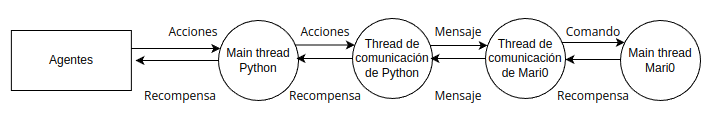
\includegraphics[width=1.0\textwidth]{img/comunication.png}
    \caption{Esquema de la alternativa por sockets[Elaboración Propia]}
    \label{fig:alternativa-1-acc}
\end{figure}


\section{Arquitectura de los mensajes}

La siguiente tarea era diseñar la arquitectura de los mensajes entre los procesos. Puesto que uno de nuestros objetivos era que el entorno fuera fácilmente adaptable, necesitábamos crear una arquitectura de mensajes fácilmente ampliable usando el paradigma de orientación a objetos. Partiendo de la base que cada agente puede ejecutar varias acciones o comandos en un mismo momento, decidimos crear la clase comando en Python.

Esta clase contendría el nombre del comando a ejecutar y los parámetros necesarios para poder ejecutarlo correctamente. A partir de esta clase creamos una jerarquía de clases. La jerarquía se divide en comandos de juego y comandos de control. Los comandos de juego se componen de los comandos que pueden ejecutar los agentes, como saltar, disparar un portal, etc. Los comandos de control se componen de las diferentes acciones que se deben aplicar para gestionar el videojuego desde el proceso de Python. En concreto son las acciones de inicializar el mapa, resetear el entorno, obtener las recompensas, cerrar el juego y observar si se ha acabado el mapa. Como podemos deducir, los comandos de recompensa y de evaluar si se ha acabado el mapa requieren que el juego envíe una respuesta. Por esto, tienen el atributo de need \_response. En Lua, decidimos crear la misma jerarquía de comandos que en Python, añadiendo además la operación Run() para implementar el funcionamiento de cada comando. En la figura \ref {fig:clases} podemos observar el esquema de la jerarquía de comandos.

\begin{figure}[ht]
    \centering
    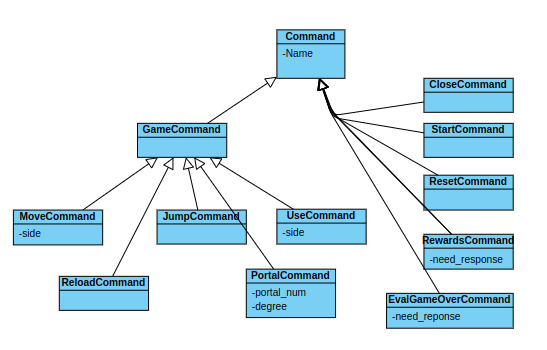
\includegraphics[width=1.0\textwidth]{img/clases.png}
    \caption{Esquema de las clases implementadas [Elaboración Propia]}
    \label{fig:clases}
\end{figure}

Adicionalmente, para facilitar el uso de estas clases, implementamos el patrón Factory, para poder obtener a partir de la lista de acciones de un agente una lista de comandos. Una vez creados los comandos, enviamos los comandos en formato JSON al videojuego. Finalmente, una vez recibido el mensaje, el videojuego lo transforma de nuevo a una lista de comandos usando el módulo de JSON de Lua y el patrón Factory y ejecuta cada comando. Podemos ver un esquema de la secuencia de operaciones en la figura \ref {fig:operations}

\begin{figure}[ht]
    \centering
    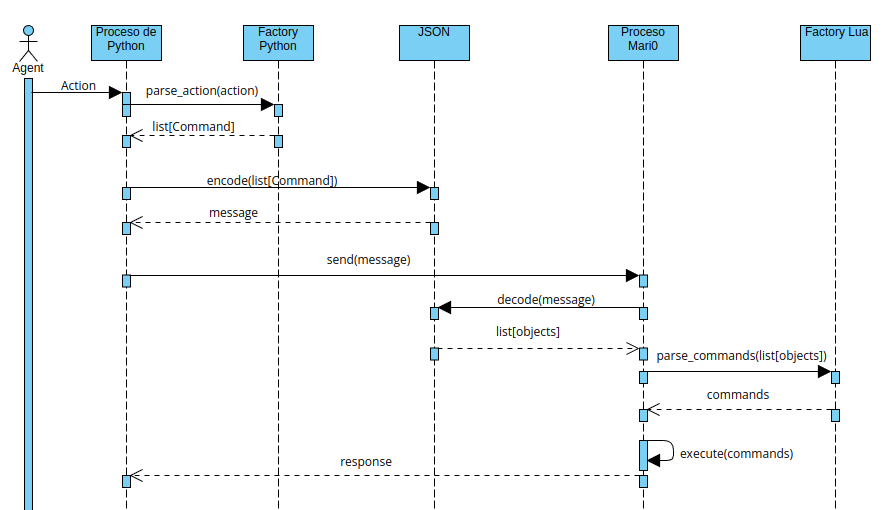
\includegraphics[width=1.0\textwidth]{img/secuencia_op.png}
    \caption{Esquema simplificado de la secuencia de operaciones en la comunicación de comandos [Elaboración Propia]}
    \label{fig:operations}
\end{figure}

Una característica a tener en consideración es que en caso de que el proceso de Python envíe un comando que requiere de respuesta, se quedará esperando a la respuesta del videojuego.

\section{Comunicación entre threads}

Otro aspecto que tuvimos que tener en cuenta fue la comunicación entre los threads. Esta comunicación se realizó en Python usando la clase cola. En concreto se crearon dos colas, una para enviar mensajes y otra para recibir las respuestas del videojuego. De forma paralela, en Lua se usaron 2 canales, que son idénticos a las colas, uno para obtener los comandos a ejecutar y otro para enviar las respuestas al entorno. En la figura \ref {fig:threads} podemos ver el esquema de la comunicación entre threads. 

\begin{figure}[ht]
    \centering
    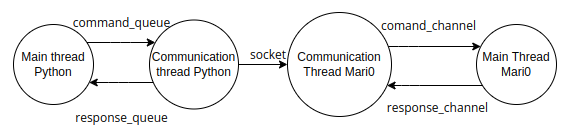
\includegraphics[width=1.0\textwidth]{img/threads.png}
    \caption{Esquema de la comunicación entre threads [Elaboración Propia]}
    \label{fig:threads}
\end{figure}

\subsection*{Problemas encontrados}

Realizando la implementación la comunicación nos encontramos con varios problemas. En esta sección explicaremos brevemente los problemas que tuvimos y su solución.

\begin{itemize}
    \item Implementación de los comandos en el juego. De los mayores problemas que hubo fue conseguir que cada comando ejecutará la operación deseada, sobretodo el principal problema consistió en el movimiento. La solución fue observar la ejecución del videojuego normal y basarse en ella para implementar los comandos.
    \item Bloqueo de los threads de comunicación. Puesto que los threads de comunicación deben coordinarse entre ellos para enviar mensajes a través de los canales o las colas y a través de los sockets, si no se gestionaba correctamente los threads se bloqueaban esperando mensajes. Además, si se llegaba al final de la ejecución del programa y los threads estaban bloqueados, todo el proceso seguía esperando de forma indefinida. Para solucionar estos problemas se implementó un tiempo de espera máximo y en caso de no obtener el mensaje esperado se continuaría normalmente con la ejecución o simplemente se cesaría la ejecución.
    \item La creación de clases y el patrón Factory en Lua. Este lenguaje no tiene un soporte propio para la orientación a objetos, aun así, es posible conseguir crear objetos similares a clases usando las propiedades del objeto básico de este lenguaje, las tablas. La solución a este problema se explicará en el siguiente apartado, al ser algo más compleja.
\end{itemize}

\subsection*{Clases en Lua}

En el lenguaje de programación Lua, además de los tipos básicos como int, string, char, etc. el único tipo complejo que existe es la tabla. Este tipo complejo es aparentemente similar a los diccionarios de Python. Puesto que no existe el concepto de clase en este lenguaje, cada objeto define su propia conducta y tiene su forma propia. Aun así, es posible crear una especie de prototipo que sirve a modo de concepto como clase. Este prototipo implementa todas las características que se buscan en la clase y cada que se quiera crear una instancia de esta clase, se informa a esta instancia que todos los métodos que esta no reconozca como propios deben buscarse en la clase prototipo. Veamos esto mejor con un ejemplo.

\begin{figure}[ht]
    \centering
    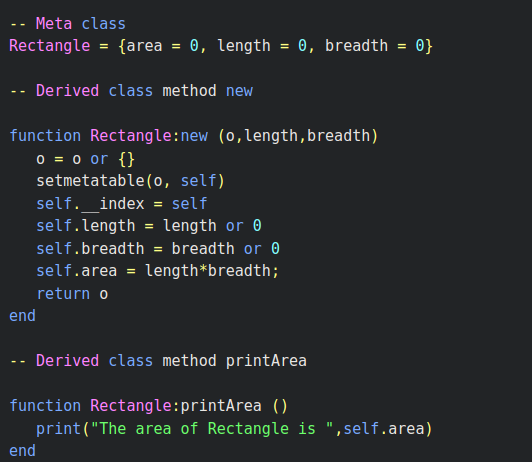
\includegraphics[width=0.8\textwidth]{img/lua-clases.png}
    \caption{Ejemplo de la creación de una clase en Lua [Elaboración Propia]}
    \label{fig:lua-clases}
\end{figure}

Supongamos que queremos crear la clase Rectangle. Esta clase tiene como parámetros el área, el ancho de la base y la altura del rectángulo. Además tiene un método que sirve para enseñar por pantalla el área de este. Para poder hacerlo, primero debemos crear el prototipo llamado Rectangle con sus parámetros. Lo siguiente que debemos hacer es crear el método de instanciación de la clase. En este método, creamos un objeto nuevo y le asignamos sus parámetros específicos. Más adelante, con la función \textbf{setmetatable} le indicamos a este objeto que cuando le sea requerido un parámetro o método que no este definido en su tabla, busque en la tabla del prototipo Rectangle. Del mismo modo, con la línea \textbf{self.index = self} indicamos que la tabla que se usará para la búsqueda es la tabla prototipo. Podemos ver la creación de esta clase en la figura \ref {fig:lua-clases}.


Con este proceso conseguiríamos crear una clase en Lua. Como se puede ver, no es un proceso trivial aun conociendo otros lenguajes de programación. De forma similar a como hemos hecho en este ejemplo, es posible crear una jerarquía de clases y una clase Factory, pero no expandiremos este proceso para no complicar excesivamente la explicación.

